\scalebox{0.55}{
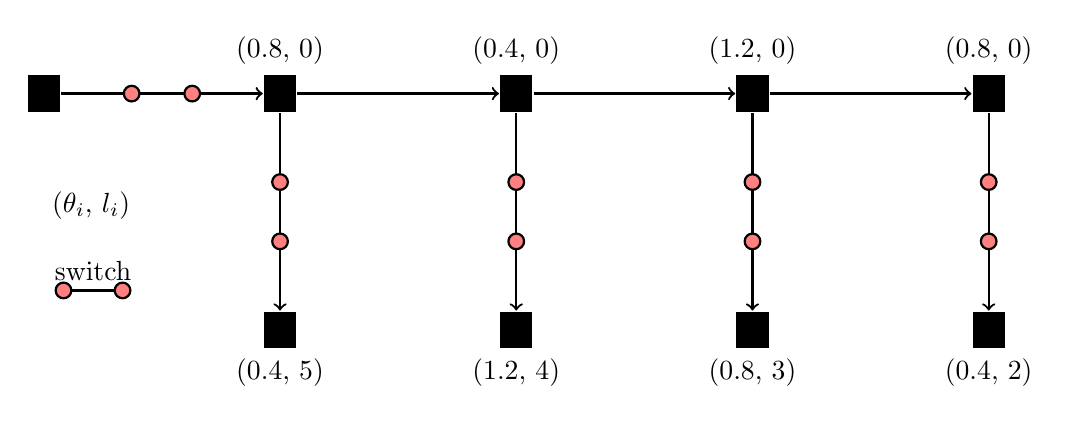
\begin{tikzpicture}
 \SetUpEdge[lw         = 1pt,
            color      = black,
            labelcolor = white]
  \GraphInit[vstyle=Normal] 
  \SetGraphUnit{3}
  \tikzset{VertexStyle/.append  style={fill,thick}}
  \tikzset{mynode/.style=VertexStyle}
  \tikzset{switch/.append style={circle,
         fill=red!50,
         thick,
         %maximum size=0.025cm,
         inner sep=2pt,
         draw},
        }
        
  \node[mynode] (0) at (0,0) {0};
  \node[mynode,label={(0.8, 0)}] (1) at (3,0) {1};
  \node[mynode,label={(0.4, 0)}] (2) at (6,0) {2};
  \node[mynode,label={(1.2, 0)}] (3) at (9,0) {3};
  \node[mynode,label={(0.8, 0)}] (4) at (12,0) {4};
  \node[mynode,label=below:{(0.4, 5)}] (5) at (3,-3) {5};
  \node[mynode,label=below:{(1.2, 4)}] (6) at (6,-3) {6};
  \node[mynode,label=below:{(0.8, 3)}] (7) at (9,-3) {7};
  \node[mynode,label=below:{(0.4, 2)}] (8) at (12,-3) {8};
  
  \node[label=below:{($\theta_i$, $l_i$)}] at (0.6,-1) {};
  \node[switch] (s1) at (0.25,-2.5) {};
  \node[switch] (s2) at (1,-2.5) {};
  \draw[thick,-,black] (s1)--(s2) node [midway,above,black] {switch};
  
  %\tikzset{EdgeStyle/.style={->}}
  \draw[thick,->,black] (0)--(1) node[pos=0.35,switch] {} node[pos=0.65,switch] {};
  %node[pos=0.65,circle,inner sep=3.5pt,draw];
  \draw[thick,->,black] (1)--(2);
  \draw[thick,->,black] (2)--(3);
  \draw[thick,->,black] (3)--(4);
  \draw[thick,->,black] (1)--(5) node[pos=0.35,switch] {} node[pos=0.65,switch] {};
  \draw[thick,->,black] (2)--(6) node[pos=0.35,switch] {} node[pos=0.65,switch] {};
  \draw[thick,->,black] (3)--(7) node[pos=0.35,switch] {} node[pos=0.65,switch] {};
  \draw[thick,->,black] (4)--(8) node[pos=0.35,switch] {} node[pos=0.65,switch] {};
\end{tikzpicture}
}